% =====================================================================
%  MSACL DS301 Deep Learning · Quiz 11 · Learning Without (Many) Labels
%  Academic problem-set style (single-source, \ifsolution toggle)
%  SINGLE SOURCE — produces BOTH the student quiz and the answer key.
%
%  ANSWER TOGGLE
%  -------------
%  Student version (answers HIDDEN) — the default:
%       pdflatex quiz11_unsupervised.tex
%  Answer key (answers SHOWN):
%       pdflatex "\def\showsolutions{}% =====================================================================
%  MSACL DS301 Deep Learning · Quiz 11 · Learning Without (Many) Labels
%  Academic problem-set style (single-source, \ifsolution toggle)
%  SINGLE SOURCE — produces BOTH the student quiz and the answer key.
%
%  ANSWER TOGGLE
%  -------------
%  Student version (answers HIDDEN) — the default:
%       pdflatex quiz11_unsupervised.tex
%  Answer key (answers SHOWN):
%       pdflatex "\def\showsolutions{}% =====================================================================
%  MSACL DS301 Deep Learning · Quiz 11 · Learning Without (Many) Labels
%  Academic problem-set style (single-source, \ifsolution toggle)
%  SINGLE SOURCE — produces BOTH the student quiz and the answer key.
%
%  ANSWER TOGGLE
%  -------------
%  Student version (answers HIDDEN) — the default:
%       pdflatex quiz11_unsupervised.tex
%  Answer key (answers SHOWN):
%       pdflatex "\def\showsolutions{}% =====================================================================
%  MSACL DS301 Deep Learning · Quiz 11 · Learning Without (Many) Labels
%  Academic problem-set style (single-source, \ifsolution toggle)
%  SINGLE SOURCE — produces BOTH the student quiz and the answer key.
%
%  ANSWER TOGGLE
%  -------------
%  Student version (answers HIDDEN) — the default:
%       pdflatex quiz11_unsupervised.tex
%  Answer key (answers SHOWN):
%       pdflatex "\def\showsolutions{}\input{quiz11_unsupervised.tex}"
%  (or, to flip by hand, change \solutionfalse to \solutiontrue below.)
% =====================================================================
\documentclass[11pt]{article}

\newif\ifsolution
\ifdefined\showsolutions \solutiontrue \else \solutionfalse \fi
% \solutiontrue   % <-- uncomment to hard-code the ANSWER KEY build

\usepackage[letterpaper, margin=0.6in, top=0.7in, bottom=0.5in]{geometry}
\usepackage{amsmath, amssymb}
\usepackage{xcolor}
\usepackage{array}
\usepackage{tikz}
\usetikzlibrary{arrows.meta, calc}
\usepackage{fancyhdr}

\pagestyle{fancy}
\fancyhf{}
\fancyhead[L]{\small\textbf{MSACL DS301 --- Deep Learning}}
\fancyhead[R]{\small\textbf{Quiz 11: Learning Without (Many) Labels\ifsolution\ \textmd{(Answer Key)}\fi}}
\fancyfoot[C]{\thepage}
\renewcommand{\headrulewidth}{0.4pt}

\newcommand{\blk}[1]{\underline{\hspace{#1}}}
% Reveal-or-blank: shows the answer in the key, a blank rule on the student sheet.
\newcommand{\rb}[2]{\ifsolution\textbf{#1}\else\blk{#2}\fi}
% Boxed answer (key only) and blank writing space (student only).
\newcommand{\keybox}[1]{\ifsolution\par\vspace{2pt}%
  \fbox{\parbox{0.965\textwidth}{\small\textbf{Answer.}\; #1}}\par\fi}
\newcommand{\work}[1]{\ifsolution\else\vspace{#1}\fi}

% ---- course palette (numeric grids / diagram) ----------------------------
\definecolor{ink}{HTML}{1B2025}
\definecolor{teal}{HTML}{0E7C7B}
\definecolor{tealsoft}{HTML}{E3F0EF}
\definecolor{amber}{HTML}{E09E2F}
\definecolor{ambersoft}{HTML}{FBF0DC}
\definecolor{redd}{HTML}{C4534F}
\definecolor{redsoft}{HTML}{F7E4E3}
\definecolor{inksoft}{HTML}{3D444C}
\definecolor{muted}{HTML}{8A9099}
\definecolor{hair}{HTML}{D9D9D2}
% square, centred, monospace cells for the numeric grids
\newcolumntype{G}{>{\centering\arraybackslash\ttfamily}p{9mm}}
\newcommand{\gr}{\renewcommand{\arraystretch}{1.5}}

\setlength{\parindent}{0pt}
\setlength{\parskip}{3pt}
\setlength{\abovedisplayskip}{5pt}
\setlength{\belowdisplayskip}{5pt}

% ---- the two latent-space pictures reproduced from the deck --------------
% Picture A = an autoencoder latent (scattered islands, big empty gaps).
% Picture B = a VAE latent (one smooth, organised, gap-free cloud).
\newcommand{\latentA}{%
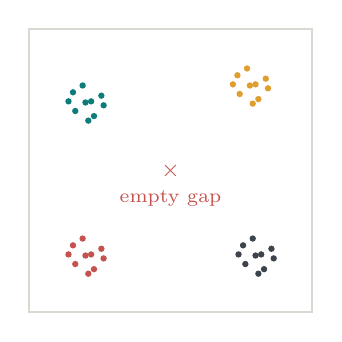
\begin{tikzpicture}[scale=0.72]
  \draw[hair, line width=0.8pt] (0,0) rectangle (5,5);
  % four tight, separated clusters with large empty gaps between them
  \foreach \cx/\cy/\col in {1/3.7/teal, 3.9/4/amber, 1/1/redd, 4/1/inksoft}{
    \foreach \dx/\dy in {0/0, 0.28/0.12, -0.22/0.18, 0.15/-0.24, -0.18/-0.15,
                         0.32/-0.05, -0.05/0.30, 0.10/0.02, -0.30/0.02, 0.05/-0.32}{
      \fill[\col] ($(\cx,\cy)+(\dx,\dy)$) circle (1.6pt);
    }
  }
  \node[redd, font=\footnotesize\bfseries] at (2.5,2.5) {$\times$};
  \node[redd, font=\scriptsize] at (2.5,2.0) {empty gap};
\end{tikzpicture}}
\newcommand{\latentB}{%
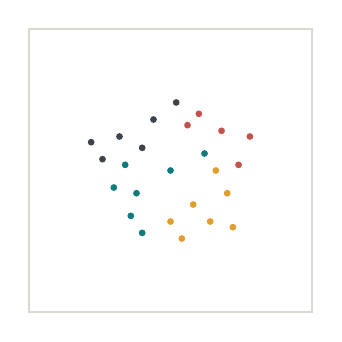
\begin{tikzpicture}[scale=0.72]
  \draw[hair, line width=0.8pt] (0,0) rectangle (5,5);
  % one broad, gap-free cloud; colours blend continuously
  \foreach \dx/\dy/\col in {%
    0/0/teal, 0.6/0.3/teal, -0.5/0.4/inksoft, 0.4/-0.6/amber, -0.6/-0.4/teal,
    0.9/0.7/redd, -0.9/0.6/inksoft, 0.7/-0.9/amber, -0.7/-0.8/teal, 1.2/0.1/redd,
    -1.2/0.2/inksoft, 0.1/1.2/inksoft, 0.2/-1.2/amber, 1.0/-0.4/amber, -1.0/-0.3/teal,
    0.3/0.8/redd, -0.3/0.9/inksoft, 0.8/0.0/amber, -0.8/0.1/teal, 0.0/-0.9/amber,
    1.4/0.6/redd, -1.4/0.5/inksoft, 0.5/1.0/redd, -0.5/-1.1/teal, 1.1/-1.0/amber}{
    \fill[\col] ($(2.5,2.5)+(\dx,\dy)$) circle (1.7pt);
  }
\end{tikzpicture}}

\begin{document}

\begin{center}
{\Large \textbf{Quiz 11 --- Learning Without (Many) Labels}}\\[2pt]
{\normalsize Predict what a latent samples to, use every spectrum, spot the reconstruction-error trap, and pick the augmentation that would corrupt contrastive pretraining}
\end{center}

\vspace{-2pt}
\begin{center}
\fbox{\parbox{0.92\textwidth}{\small
\textbf{Instructions:}\; Answer all four questions --- every part is answerable from the
pictures and rules on the slides. Intuition first; the only arithmetic is a mean of three
squared numbers. No calculators needed.%
\ifsolution\else\\[4pt]\textbf{Name:}\ \blk{6cm}\hfill\textbf{Date:}\ \blk{3.5cm}\fi
}}
\end{center}

\vspace{-2pt}\hrule\vspace{5pt}

% =========================== Q1 ===========================
\textbf{1. Sample each latent --- what decodes?}\; {\small Below are two latent-space maps of the
\emph{same} spectra --- the pair you saw on the slides. You want to \textbf{generate synthetic
resistant spectra} to augment training, so you sample a \emph{random} latent point and decode it.}

\vspace{4pt}
\begin{center}
\begin{tabular}{cc}
\latentA & \latentB \\[2pt]
\textbf{Picture A} & \textbf{Picture B}
\end{tabular}
\end{center}

\vspace{2pt}
\textbf{(a)} Sample \& decode a random point from \textbf{Picture A} (islands with gaps) --- what
comes out, and why?\hfill $\rightarrow$\; \rb{garbage (lands in an empty gap)}{5.6cm}

\vspace{3pt}
\textbf{(b)} Sample \& decode from \textbf{Picture B} (one smooth cloud) --- what comes out?
\hfill $\rightarrow$\; \rb{a plausible spectrum}{5.0cm}

\vspace{3pt}
\textbf{(c)} Which picture is the \textbf{VAE}, and which latent do you use to generate?
\hfill $\rightarrow$\; \rb{Picture B (the VAE)}{4.4cm}

\work{0.4cm}

\keybox{(a) \textbf{Garbage / a non-physical spectrum.} Picture A is a plain autoencoder: its
latent is scattered islands with big empty \textbf{gaps}, so a random sample lands where the
decoder was never trained. (b) \textbf{A plausible spectrum} --- Picture B is one smooth,
gap-free cloud, so \emph{every} point decodes to something realistic. (c) \textbf{Picture B is
the VAE}, and it is the latent you sample to generate (or interpolate): only a gap-free latent
is safe to sample. (B is also the map you would trust to flag a \emph{novel} contaminant --- a
genuinely new spectrum lands outside the tidy cloud, easy to flag.)}

\vspace{2pt}\hrule\vspace{5pt}

% =========================== Q2 ===========================
\textbf{2. Use every spectrum --- decide.}\; {\small You have \textbf{300 labelled} spectra
(susceptible/resistant known) and \textbf{40{,}000 unlabelled} QC runs, and you want a resistance
classifier. Use the four-paradigm chart from the slides.}

\vspace{4pt}
\textbf{(a)} Which paradigm uses \emph{all} of your data?\hfill $\rightarrow$\;\rb{semi-supervised}{4.6cm}

\vspace{3pt}
\textbf{(b)} Name the specific technique.\hfill $\rightarrow$\;\rb{pseudo-labelling}{4.6cm}

\vspace{3pt}
\textbf{(c)} In one sentence, the \emph{failure mode} to watch?

\work{1.0cm}
\ifsolution\else\blk{\linewidth}\fi

\keybox{(a) \textbf{Semi-supervised} --- a few labels plus many unlabelled examples, so use both
(the middle path). (b) \textbf{Pseudo-labelling}: train a first model on the 300 labelled,
predict on the 40{,}000 unlabelled, keep only the \emph{confident} predictions as pseudo-labels,
and retrain on the combined set (optionally repeat). (c) \textbf{Confident-but-wrong pseudo-labels
reinforce the model's own mistakes} --- a weak early model can poison the pool, so the confidence
filter matters. (Pure supervised would throw away 40{,}000 runs; pure unsupervised would ignore
the 300 labels you paid for.)}

\vspace{2pt}\hrule\vspace{5pt}

% =========================== Q3 ===========================
\textbf{3. Reconstruction error --- the aggregation trap.}\; {\small An autoencoder trained on
\emph{good} runs reconstructs a new spectrum of \textbf{20 $m/z$ bins}. A contaminant spikes
exactly \textbf{one} bin: that bin's squared error is \textbf{0.40}; the other \textbf{19} bins
reconstruct perfectly (error 0). Reconstruction error is the \emph{mean} squared error}
\[
  \text{MSE} \;=\; \tfrac{1}{n}\sum_{i}\,(x_i-\hat{x}_i)^2 ,
  \qquad\text{{\small flag an \textbf{anomaly} if the error } } > 0.05 .
\]

\vspace{2pt}
\textbf{(a)} MEAN over all 20 bins: $\text{MSE} = 0.40 / 20 = $ \rb{$0.02$}{2.0cm}

\work{0.4cm}

\textbf{(b)} Using the \emph{mean} and threshold $0.05$, does it flag the run?
\hfill $\rightarrow$\; \rb{no --- $0.02 < 0.05$, it PASSES}{5.4cm}

\work{0.4cm}

\textbf{(c)} The mean just \emph{missed} a real contaminant. Which \emph{single} number would have
caught it, and why does averaging hide a one-bin spike?

\work{1.1cm}
\ifsolution\else\blk{\linewidth}\\[6pt]\blk{\linewidth}\fi

\keybox{(a) $\text{MSE}=0.40/20=\mathbf{0.02}$. (b) \textbf{No} --- $0.02 < 0.05$, so the mean-MSE
\textbf{passes} the run and the contaminant slips through. (c) The \textbf{MAX per-bin error}
($0.40 > 0.05$), or the error inside the peak window, would flag it. The mean divides one big
error across 20 bins, so a \emph{localized} spike is diluted below threshold --- over thousands of
real $m/z$ bins a single contaminant peak can vanish into the average. Lesson: match the anomaly
\emph{score} to the anomaly's shape, and set the threshold as the same sensitivity/specificity
dial as Lecture~10.}

\vspace{2pt}\hrule\vspace{5pt}

% =========================== Q4 ===========================
\textbf{4. Which augmentation would corrupt it?}\; {\small Contrastive pretraining forces two
\emph{augmented views} of the \emph{same} spectrum to land at the \textbf{same} point in embedding
space. Three of the augmentations below are fine; \textbf{one} would corrupt the training.}

\vspace{3pt}
Mark each \textbf{SAFE} or \textbf{CORRUPT}:

\vspace{2pt}
(a) add random intensity noise $\rightarrow$ \rb{SAFE}{2.6cm} \qquad
(b) shift the $m/z$ axis by $0.2$ Da $\rightarrow$ \rb{SAFE}{2.6cm}

\vspace{2pt}
(c) replace it with a \emph{different} patient's spectrum $\rightarrow$ \rb{\textbf{CORRUPT}}{2.6cm} \qquad
(d) scale all intensities by $\times 1.05$ $\rightarrow$ \rb{SAFE}{2.6cm}

\vspace{3pt}
Which one is corrupt, and in one sentence, what would forcing agreement then teach the model?

\work{1.0cm}
\ifsolution\else\blk{\linewidth}\\[6pt]\blk{\linewidth}\fi

\keybox{\textbf{(c) is corrupt}; (a), (b) and (d) are safe. A valid augmentation adds only the
\emph{nuisance} variation the SAME sample would show run-to-run --- detector noise, a small $m/z$
calibration drift, a global intensity rescale --- so forcing those views to agree makes the model
\textbf{ignore the nuisance and keep the real content} (augmentation-invariance). But (c) is a
\emph{genuinely different sample}: forcing its embedding to match would teach the model to
\textbf{ignore real biological differences} --- it would treat two different patients as identical.
Rule: augmentations must preserve the underlying biology.}

\vspace{4pt}\hrule\vspace{3pt}
{\small\itshape \ifsolution Answer key.\else Keep this sheet --- Lab 4 trains a real VAE on
spectra, scores anomalies by reconstruction error, and plots the latent map.\fi}

\end{document}
"
%  (or, to flip by hand, change \solutionfalse to \solutiontrue below.)
% =====================================================================
\documentclass[11pt]{article}

\newif\ifsolution
\ifdefined\showsolutions \solutiontrue \else \solutionfalse \fi
% \solutiontrue   % <-- uncomment to hard-code the ANSWER KEY build

\usepackage[letterpaper, margin=0.6in, top=0.7in, bottom=0.5in]{geometry}
\usepackage{amsmath, amssymb}
\usepackage{xcolor}
\usepackage{array}
\usepackage{tikz}
\usetikzlibrary{arrows.meta, calc}
\usepackage{fancyhdr}

\pagestyle{fancy}
\fancyhf{}
\fancyhead[L]{\small\textbf{MSACL DS301 --- Deep Learning}}
\fancyhead[R]{\small\textbf{Quiz 11: Learning Without (Many) Labels\ifsolution\ \textmd{(Answer Key)}\fi}}
\fancyfoot[C]{\thepage}
\renewcommand{\headrulewidth}{0.4pt}

\newcommand{\blk}[1]{\underline{\hspace{#1}}}
% Reveal-or-blank: shows the answer in the key, a blank rule on the student sheet.
\newcommand{\rb}[2]{\ifsolution\textbf{#1}\else\blk{#2}\fi}
% Boxed answer (key only) and blank writing space (student only).
\newcommand{\keybox}[1]{\ifsolution\par\vspace{2pt}%
  \fbox{\parbox{0.965\textwidth}{\small\textbf{Answer.}\; #1}}\par\fi}
\newcommand{\work}[1]{\ifsolution\else\vspace{#1}\fi}

% ---- course palette (numeric grids / diagram) ----------------------------
\definecolor{ink}{HTML}{1B2025}
\definecolor{teal}{HTML}{0E7C7B}
\definecolor{tealsoft}{HTML}{E3F0EF}
\definecolor{amber}{HTML}{E09E2F}
\definecolor{ambersoft}{HTML}{FBF0DC}
\definecolor{redd}{HTML}{C4534F}
\definecolor{redsoft}{HTML}{F7E4E3}
\definecolor{inksoft}{HTML}{3D444C}
\definecolor{muted}{HTML}{8A9099}
\definecolor{hair}{HTML}{D9D9D2}
% square, centred, monospace cells for the numeric grids
\newcolumntype{G}{>{\centering\arraybackslash\ttfamily}p{9mm}}
\newcommand{\gr}{\renewcommand{\arraystretch}{1.5}}

\setlength{\parindent}{0pt}
\setlength{\parskip}{3pt}
\setlength{\abovedisplayskip}{5pt}
\setlength{\belowdisplayskip}{5pt}

% ---- the two latent-space pictures reproduced from the deck --------------
% Picture A = an autoencoder latent (scattered islands, big empty gaps).
% Picture B = a VAE latent (one smooth, organised, gap-free cloud).
\newcommand{\latentA}{%
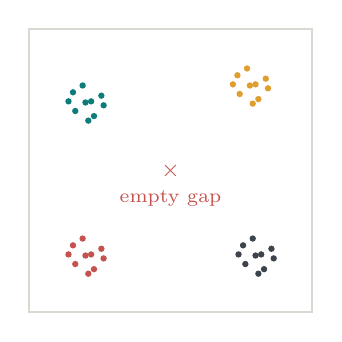
\begin{tikzpicture}[scale=0.72]
  \draw[hair, line width=0.8pt] (0,0) rectangle (5,5);
  % four tight, separated clusters with large empty gaps between them
  \foreach \cx/\cy/\col in {1/3.7/teal, 3.9/4/amber, 1/1/redd, 4/1/inksoft}{
    \foreach \dx/\dy in {0/0, 0.28/0.12, -0.22/0.18, 0.15/-0.24, -0.18/-0.15,
                         0.32/-0.05, -0.05/0.30, 0.10/0.02, -0.30/0.02, 0.05/-0.32}{
      \fill[\col] ($(\cx,\cy)+(\dx,\dy)$) circle (1.6pt);
    }
  }
  \node[redd, font=\footnotesize\bfseries] at (2.5,2.5) {$\times$};
  \node[redd, font=\scriptsize] at (2.5,2.0) {empty gap};
\end{tikzpicture}}
\newcommand{\latentB}{%
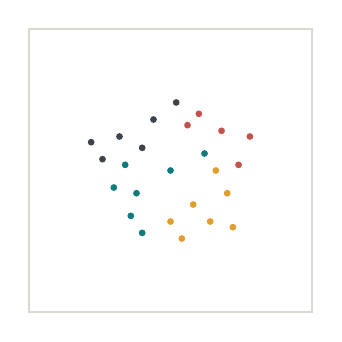
\begin{tikzpicture}[scale=0.72]
  \draw[hair, line width=0.8pt] (0,0) rectangle (5,5);
  % one broad, gap-free cloud; colours blend continuously
  \foreach \dx/\dy/\col in {%
    0/0/teal, 0.6/0.3/teal, -0.5/0.4/inksoft, 0.4/-0.6/amber, -0.6/-0.4/teal,
    0.9/0.7/redd, -0.9/0.6/inksoft, 0.7/-0.9/amber, -0.7/-0.8/teal, 1.2/0.1/redd,
    -1.2/0.2/inksoft, 0.1/1.2/inksoft, 0.2/-1.2/amber, 1.0/-0.4/amber, -1.0/-0.3/teal,
    0.3/0.8/redd, -0.3/0.9/inksoft, 0.8/0.0/amber, -0.8/0.1/teal, 0.0/-0.9/amber,
    1.4/0.6/redd, -1.4/0.5/inksoft, 0.5/1.0/redd, -0.5/-1.1/teal, 1.1/-1.0/amber}{
    \fill[\col] ($(2.5,2.5)+(\dx,\dy)$) circle (1.7pt);
  }
\end{tikzpicture}}

\begin{document}

\begin{center}
{\Large \textbf{Quiz 11 --- Learning Without (Many) Labels}}\\[2pt]
{\normalsize Predict what a latent samples to, use every spectrum, spot the reconstruction-error trap, and pick the augmentation that would corrupt contrastive pretraining}
\end{center}

\vspace{-2pt}
\begin{center}
\fbox{\parbox{0.92\textwidth}{\small
\textbf{Instructions:}\; Answer all four questions --- every part is answerable from the
pictures and rules on the slides. Intuition first; the only arithmetic is a mean of three
squared numbers. No calculators needed.%
\ifsolution\else\\[4pt]\textbf{Name:}\ \blk{6cm}\hfill\textbf{Date:}\ \blk{3.5cm}\fi
}}
\end{center}

\vspace{-2pt}\hrule\vspace{5pt}

% =========================== Q1 ===========================
\textbf{1. Sample each latent --- what decodes?}\; {\small Below are two latent-space maps of the
\emph{same} spectra --- the pair you saw on the slides. You want to \textbf{generate synthetic
resistant spectra} to augment training, so you sample a \emph{random} latent point and decode it.}

\vspace{4pt}
\begin{center}
\begin{tabular}{cc}
\latentA & \latentB \\[2pt]
\textbf{Picture A} & \textbf{Picture B}
\end{tabular}
\end{center}

\vspace{2pt}
\textbf{(a)} Sample \& decode a random point from \textbf{Picture A} (islands with gaps) --- what
comes out, and why?\hfill $\rightarrow$\; \rb{garbage (lands in an empty gap)}{5.6cm}

\vspace{3pt}
\textbf{(b)} Sample \& decode from \textbf{Picture B} (one smooth cloud) --- what comes out?
\hfill $\rightarrow$\; \rb{a plausible spectrum}{5.0cm}

\vspace{3pt}
\textbf{(c)} Which picture is the \textbf{VAE}, and which latent do you use to generate?
\hfill $\rightarrow$\; \rb{Picture B (the VAE)}{4.4cm}

\work{0.4cm}

\keybox{(a) \textbf{Garbage / a non-physical spectrum.} Picture A is a plain autoencoder: its
latent is scattered islands with big empty \textbf{gaps}, so a random sample lands where the
decoder was never trained. (b) \textbf{A plausible spectrum} --- Picture B is one smooth,
gap-free cloud, so \emph{every} point decodes to something realistic. (c) \textbf{Picture B is
the VAE}, and it is the latent you sample to generate (or interpolate): only a gap-free latent
is safe to sample. (B is also the map you would trust to flag a \emph{novel} contaminant --- a
genuinely new spectrum lands outside the tidy cloud, easy to flag.)}

\vspace{2pt}\hrule\vspace{5pt}

% =========================== Q2 ===========================
\textbf{2. Use every spectrum --- decide.}\; {\small You have \textbf{300 labelled} spectra
(susceptible/resistant known) and \textbf{40{,}000 unlabelled} QC runs, and you want a resistance
classifier. Use the four-paradigm chart from the slides.}

\vspace{4pt}
\textbf{(a)} Which paradigm uses \emph{all} of your data?\hfill $\rightarrow$\;\rb{semi-supervised}{4.6cm}

\vspace{3pt}
\textbf{(b)} Name the specific technique.\hfill $\rightarrow$\;\rb{pseudo-labelling}{4.6cm}

\vspace{3pt}
\textbf{(c)} In one sentence, the \emph{failure mode} to watch?

\work{1.0cm}
\ifsolution\else\blk{\linewidth}\fi

\keybox{(a) \textbf{Semi-supervised} --- a few labels plus many unlabelled examples, so use both
(the middle path). (b) \textbf{Pseudo-labelling}: train a first model on the 300 labelled,
predict on the 40{,}000 unlabelled, keep only the \emph{confident} predictions as pseudo-labels,
and retrain on the combined set (optionally repeat). (c) \textbf{Confident-but-wrong pseudo-labels
reinforce the model's own mistakes} --- a weak early model can poison the pool, so the confidence
filter matters. (Pure supervised would throw away 40{,}000 runs; pure unsupervised would ignore
the 300 labels you paid for.)}

\vspace{2pt}\hrule\vspace{5pt}

% =========================== Q3 ===========================
\textbf{3. Reconstruction error --- the aggregation trap.}\; {\small An autoencoder trained on
\emph{good} runs reconstructs a new spectrum of \textbf{20 $m/z$ bins}. A contaminant spikes
exactly \textbf{one} bin: that bin's squared error is \textbf{0.40}; the other \textbf{19} bins
reconstruct perfectly (error 0). Reconstruction error is the \emph{mean} squared error}
\[
  \text{MSE} \;=\; \tfrac{1}{n}\sum_{i}\,(x_i-\hat{x}_i)^2 ,
  \qquad\text{{\small flag an \textbf{anomaly} if the error } } > 0.05 .
\]

\vspace{2pt}
\textbf{(a)} MEAN over all 20 bins: $\text{MSE} = 0.40 / 20 = $ \rb{$0.02$}{2.0cm}

\work{0.4cm}

\textbf{(b)} Using the \emph{mean} and threshold $0.05$, does it flag the run?
\hfill $\rightarrow$\; \rb{no --- $0.02 < 0.05$, it PASSES}{5.4cm}

\work{0.4cm}

\textbf{(c)} The mean just \emph{missed} a real contaminant. Which \emph{single} number would have
caught it, and why does averaging hide a one-bin spike?

\work{1.1cm}
\ifsolution\else\blk{\linewidth}\\[6pt]\blk{\linewidth}\fi

\keybox{(a) $\text{MSE}=0.40/20=\mathbf{0.02}$. (b) \textbf{No} --- $0.02 < 0.05$, so the mean-MSE
\textbf{passes} the run and the contaminant slips through. (c) The \textbf{MAX per-bin error}
($0.40 > 0.05$), or the error inside the peak window, would flag it. The mean divides one big
error across 20 bins, so a \emph{localized} spike is diluted below threshold --- over thousands of
real $m/z$ bins a single contaminant peak can vanish into the average. Lesson: match the anomaly
\emph{score} to the anomaly's shape, and set the threshold as the same sensitivity/specificity
dial as Lecture~10.}

\vspace{2pt}\hrule\vspace{5pt}

% =========================== Q4 ===========================
\textbf{4. Which augmentation would corrupt it?}\; {\small Contrastive pretraining forces two
\emph{augmented views} of the \emph{same} spectrum to land at the \textbf{same} point in embedding
space. Three of the augmentations below are fine; \textbf{one} would corrupt the training.}

\vspace{3pt}
Mark each \textbf{SAFE} or \textbf{CORRUPT}:

\vspace{2pt}
(a) add random intensity noise $\rightarrow$ \rb{SAFE}{2.6cm} \qquad
(b) shift the $m/z$ axis by $0.2$ Da $\rightarrow$ \rb{SAFE}{2.6cm}

\vspace{2pt}
(c) replace it with a \emph{different} patient's spectrum $\rightarrow$ \rb{\textbf{CORRUPT}}{2.6cm} \qquad
(d) scale all intensities by $\times 1.05$ $\rightarrow$ \rb{SAFE}{2.6cm}

\vspace{3pt}
Which one is corrupt, and in one sentence, what would forcing agreement then teach the model?

\work{1.0cm}
\ifsolution\else\blk{\linewidth}\\[6pt]\blk{\linewidth}\fi

\keybox{\textbf{(c) is corrupt}; (a), (b) and (d) are safe. A valid augmentation adds only the
\emph{nuisance} variation the SAME sample would show run-to-run --- detector noise, a small $m/z$
calibration drift, a global intensity rescale --- so forcing those views to agree makes the model
\textbf{ignore the nuisance and keep the real content} (augmentation-invariance). But (c) is a
\emph{genuinely different sample}: forcing its embedding to match would teach the model to
\textbf{ignore real biological differences} --- it would treat two different patients as identical.
Rule: augmentations must preserve the underlying biology.}

\vspace{4pt}\hrule\vspace{3pt}
{\small\itshape \ifsolution Answer key.\else Keep this sheet --- Lab 4 trains a real VAE on
spectra, scores anomalies by reconstruction error, and plots the latent map.\fi}

\end{document}
"
%  (or, to flip by hand, change \solutionfalse to \solutiontrue below.)
% =====================================================================
\documentclass[11pt]{article}

\newif\ifsolution
\ifdefined\showsolutions \solutiontrue \else \solutionfalse \fi
% \solutiontrue   % <-- uncomment to hard-code the ANSWER KEY build

\usepackage[letterpaper, margin=0.6in, top=0.7in, bottom=0.5in]{geometry}
\usepackage{amsmath, amssymb}
\usepackage{xcolor}
\usepackage{array}
\usepackage{tikz}
\usetikzlibrary{arrows.meta, calc}
\usepackage{fancyhdr}

\pagestyle{fancy}
\fancyhf{}
\fancyhead[L]{\small\textbf{MSACL DS301 --- Deep Learning}}
\fancyhead[R]{\small\textbf{Quiz 11: Learning Without (Many) Labels\ifsolution\ \textmd{(Answer Key)}\fi}}
\fancyfoot[C]{\thepage}
\renewcommand{\headrulewidth}{0.4pt}

\newcommand{\blk}[1]{\underline{\hspace{#1}}}
% Reveal-or-blank: shows the answer in the key, a blank rule on the student sheet.
\newcommand{\rb}[2]{\ifsolution\textbf{#1}\else\blk{#2}\fi}
% Boxed answer (key only) and blank writing space (student only).
\newcommand{\keybox}[1]{\ifsolution\par\vspace{2pt}%
  \fbox{\parbox{0.965\textwidth}{\small\textbf{Answer.}\; #1}}\par\fi}
\newcommand{\work}[1]{\ifsolution\else\vspace{#1}\fi}

% ---- course palette (numeric grids / diagram) ----------------------------
\definecolor{ink}{HTML}{1B2025}
\definecolor{teal}{HTML}{0E7C7B}
\definecolor{tealsoft}{HTML}{E3F0EF}
\definecolor{amber}{HTML}{E09E2F}
\definecolor{ambersoft}{HTML}{FBF0DC}
\definecolor{redd}{HTML}{C4534F}
\definecolor{redsoft}{HTML}{F7E4E3}
\definecolor{inksoft}{HTML}{3D444C}
\definecolor{muted}{HTML}{8A9099}
\definecolor{hair}{HTML}{D9D9D2}
% square, centred, monospace cells for the numeric grids
\newcolumntype{G}{>{\centering\arraybackslash\ttfamily}p{9mm}}
\newcommand{\gr}{\renewcommand{\arraystretch}{1.5}}

\setlength{\parindent}{0pt}
\setlength{\parskip}{3pt}
\setlength{\abovedisplayskip}{5pt}
\setlength{\belowdisplayskip}{5pt}

% ---- the two latent-space pictures reproduced from the deck --------------
% Picture A = an autoencoder latent (scattered islands, big empty gaps).
% Picture B = a VAE latent (one smooth, organised, gap-free cloud).
\newcommand{\latentA}{%
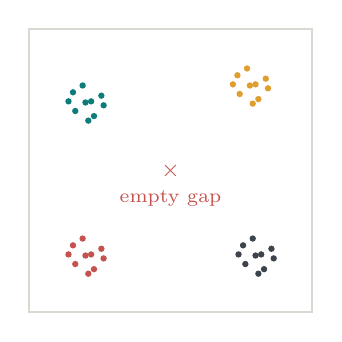
\begin{tikzpicture}[scale=0.72]
  \draw[hair, line width=0.8pt] (0,0) rectangle (5,5);
  % four tight, separated clusters with large empty gaps between them
  \foreach \cx/\cy/\col in {1/3.7/teal, 3.9/4/amber, 1/1/redd, 4/1/inksoft}{
    \foreach \dx/\dy in {0/0, 0.28/0.12, -0.22/0.18, 0.15/-0.24, -0.18/-0.15,
                         0.32/-0.05, -0.05/0.30, 0.10/0.02, -0.30/0.02, 0.05/-0.32}{
      \fill[\col] ($(\cx,\cy)+(\dx,\dy)$) circle (1.6pt);
    }
  }
  \node[redd, font=\footnotesize\bfseries] at (2.5,2.5) {$\times$};
  \node[redd, font=\scriptsize] at (2.5,2.0) {empty gap};
\end{tikzpicture}}
\newcommand{\latentB}{%
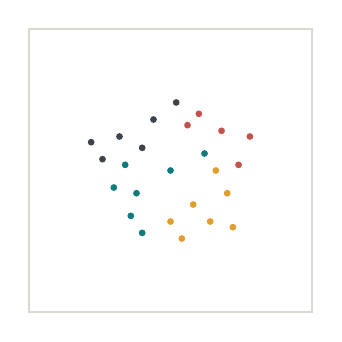
\begin{tikzpicture}[scale=0.72]
  \draw[hair, line width=0.8pt] (0,0) rectangle (5,5);
  % one broad, gap-free cloud; colours blend continuously
  \foreach \dx/\dy/\col in {%
    0/0/teal, 0.6/0.3/teal, -0.5/0.4/inksoft, 0.4/-0.6/amber, -0.6/-0.4/teal,
    0.9/0.7/redd, -0.9/0.6/inksoft, 0.7/-0.9/amber, -0.7/-0.8/teal, 1.2/0.1/redd,
    -1.2/0.2/inksoft, 0.1/1.2/inksoft, 0.2/-1.2/amber, 1.0/-0.4/amber, -1.0/-0.3/teal,
    0.3/0.8/redd, -0.3/0.9/inksoft, 0.8/0.0/amber, -0.8/0.1/teal, 0.0/-0.9/amber,
    1.4/0.6/redd, -1.4/0.5/inksoft, 0.5/1.0/redd, -0.5/-1.1/teal, 1.1/-1.0/amber}{
    \fill[\col] ($(2.5,2.5)+(\dx,\dy)$) circle (1.7pt);
  }
\end{tikzpicture}}

\begin{document}

\begin{center}
{\Large \textbf{Quiz 11 --- Learning Without (Many) Labels}}\\[2pt]
{\normalsize Predict what a latent samples to, use every spectrum, spot the reconstruction-error trap, and pick the augmentation that would corrupt contrastive pretraining}
\end{center}

\vspace{-2pt}
\begin{center}
\fbox{\parbox{0.92\textwidth}{\small
\textbf{Instructions:}\; Answer all four questions --- every part is answerable from the
pictures and rules on the slides. Intuition first; the only arithmetic is a mean of three
squared numbers. No calculators needed.%
\ifsolution\else\\[4pt]\textbf{Name:}\ \blk{6cm}\hfill\textbf{Date:}\ \blk{3.5cm}\fi
}}
\end{center}

\vspace{-2pt}\hrule\vspace{5pt}

% =========================== Q1 ===========================
\textbf{1. Sample each latent --- what decodes?}\; {\small Below are two latent-space maps of the
\emph{same} spectra --- the pair you saw on the slides. You want to \textbf{generate synthetic
resistant spectra} to augment training, so you sample a \emph{random} latent point and decode it.}

\vspace{4pt}
\begin{center}
\begin{tabular}{cc}
\latentA & \latentB \\[2pt]
\textbf{Picture A} & \textbf{Picture B}
\end{tabular}
\end{center}

\vspace{2pt}
\textbf{(a)} Sample \& decode a random point from \textbf{Picture A} (islands with gaps) --- what
comes out, and why?\hfill $\rightarrow$\; \rb{garbage (lands in an empty gap)}{5.6cm}

\vspace{3pt}
\textbf{(b)} Sample \& decode from \textbf{Picture B} (one smooth cloud) --- what comes out?
\hfill $\rightarrow$\; \rb{a plausible spectrum}{5.0cm}

\vspace{3pt}
\textbf{(c)} Which picture is the \textbf{VAE}, and which latent do you use to generate?
\hfill $\rightarrow$\; \rb{Picture B (the VAE)}{4.4cm}

\work{0.4cm}

\keybox{(a) \textbf{Garbage / a non-physical spectrum.} Picture A is a plain autoencoder: its
latent is scattered islands with big empty \textbf{gaps}, so a random sample lands where the
decoder was never trained. (b) \textbf{A plausible spectrum} --- Picture B is one smooth,
gap-free cloud, so \emph{every} point decodes to something realistic. (c) \textbf{Picture B is
the VAE}, and it is the latent you sample to generate (or interpolate): only a gap-free latent
is safe to sample. (B is also the map you would trust to flag a \emph{novel} contaminant --- a
genuinely new spectrum lands outside the tidy cloud, easy to flag.)}

\vspace{2pt}\hrule\vspace{5pt}

% =========================== Q2 ===========================
\textbf{2. Use every spectrum --- decide.}\; {\small You have \textbf{300 labelled} spectra
(susceptible/resistant known) and \textbf{40{,}000 unlabelled} QC runs, and you want a resistance
classifier. Use the four-paradigm chart from the slides.}

\vspace{4pt}
\textbf{(a)} Which paradigm uses \emph{all} of your data?\hfill $\rightarrow$\;\rb{semi-supervised}{4.6cm}

\vspace{3pt}
\textbf{(b)} Name the specific technique.\hfill $\rightarrow$\;\rb{pseudo-labelling}{4.6cm}

\vspace{3pt}
\textbf{(c)} In one sentence, the \emph{failure mode} to watch?

\work{1.0cm}
\ifsolution\else\blk{\linewidth}\fi

\keybox{(a) \textbf{Semi-supervised} --- a few labels plus many unlabelled examples, so use both
(the middle path). (b) \textbf{Pseudo-labelling}: train a first model on the 300 labelled,
predict on the 40{,}000 unlabelled, keep only the \emph{confident} predictions as pseudo-labels,
and retrain on the combined set (optionally repeat). (c) \textbf{Confident-but-wrong pseudo-labels
reinforce the model's own mistakes} --- a weak early model can poison the pool, so the confidence
filter matters. (Pure supervised would throw away 40{,}000 runs; pure unsupervised would ignore
the 300 labels you paid for.)}

\vspace{2pt}\hrule\vspace{5pt}

% =========================== Q3 ===========================
\textbf{3. Reconstruction error --- the aggregation trap.}\; {\small An autoencoder trained on
\emph{good} runs reconstructs a new spectrum of \textbf{20 $m/z$ bins}. A contaminant spikes
exactly \textbf{one} bin: that bin's squared error is \textbf{0.40}; the other \textbf{19} bins
reconstruct perfectly (error 0). Reconstruction error is the \emph{mean} squared error}
\[
  \text{MSE} \;=\; \tfrac{1}{n}\sum_{i}\,(x_i-\hat{x}_i)^2 ,
  \qquad\text{{\small flag an \textbf{anomaly} if the error } } > 0.05 .
\]

\vspace{2pt}
\textbf{(a)} MEAN over all 20 bins: $\text{MSE} = 0.40 / 20 = $ \rb{$0.02$}{2.0cm}

\work{0.4cm}

\textbf{(b)} Using the \emph{mean} and threshold $0.05$, does it flag the run?
\hfill $\rightarrow$\; \rb{no --- $0.02 < 0.05$, it PASSES}{5.4cm}

\work{0.4cm}

\textbf{(c)} The mean just \emph{missed} a real contaminant. Which \emph{single} number would have
caught it, and why does averaging hide a one-bin spike?

\work{1.1cm}
\ifsolution\else\blk{\linewidth}\\[6pt]\blk{\linewidth}\fi

\keybox{(a) $\text{MSE}=0.40/20=\mathbf{0.02}$. (b) \textbf{No} --- $0.02 < 0.05$, so the mean-MSE
\textbf{passes} the run and the contaminant slips through. (c) The \textbf{MAX per-bin error}
($0.40 > 0.05$), or the error inside the peak window, would flag it. The mean divides one big
error across 20 bins, so a \emph{localized} spike is diluted below threshold --- over thousands of
real $m/z$ bins a single contaminant peak can vanish into the average. Lesson: match the anomaly
\emph{score} to the anomaly's shape, and set the threshold as the same sensitivity/specificity
dial as Lecture~10.}

\vspace{2pt}\hrule\vspace{5pt}

% =========================== Q4 ===========================
\textbf{4. Which augmentation would corrupt it?}\; {\small Contrastive pretraining forces two
\emph{augmented views} of the \emph{same} spectrum to land at the \textbf{same} point in embedding
space. Three of the augmentations below are fine; \textbf{one} would corrupt the training.}

\vspace{3pt}
Mark each \textbf{SAFE} or \textbf{CORRUPT}:

\vspace{2pt}
(a) add random intensity noise $\rightarrow$ \rb{SAFE}{2.6cm} \qquad
(b) shift the $m/z$ axis by $0.2$ Da $\rightarrow$ \rb{SAFE}{2.6cm}

\vspace{2pt}
(c) replace it with a \emph{different} patient's spectrum $\rightarrow$ \rb{\textbf{CORRUPT}}{2.6cm} \qquad
(d) scale all intensities by $\times 1.05$ $\rightarrow$ \rb{SAFE}{2.6cm}

\vspace{3pt}
Which one is corrupt, and in one sentence, what would forcing agreement then teach the model?

\work{1.0cm}
\ifsolution\else\blk{\linewidth}\\[6pt]\blk{\linewidth}\fi

\keybox{\textbf{(c) is corrupt}; (a), (b) and (d) are safe. A valid augmentation adds only the
\emph{nuisance} variation the SAME sample would show run-to-run --- detector noise, a small $m/z$
calibration drift, a global intensity rescale --- so forcing those views to agree makes the model
\textbf{ignore the nuisance and keep the real content} (augmentation-invariance). But (c) is a
\emph{genuinely different sample}: forcing its embedding to match would teach the model to
\textbf{ignore real biological differences} --- it would treat two different patients as identical.
Rule: augmentations must preserve the underlying biology.}

\vspace{4pt}\hrule\vspace{3pt}
{\small\itshape \ifsolution Answer key.\else Keep this sheet --- Lab 4 trains a real VAE on
spectra, scores anomalies by reconstruction error, and plots the latent map.\fi}

\end{document}
"
%  (or, to flip by hand, change \solutionfalse to \solutiontrue below.)
% =====================================================================
\documentclass[11pt]{article}

\newif\ifsolution
\ifdefined\showsolutions \solutiontrue \else \solutionfalse \fi
% \solutiontrue   % <-- uncomment to hard-code the ANSWER KEY build

\usepackage[letterpaper, margin=0.6in, top=0.7in, bottom=0.5in]{geometry}
\usepackage{amsmath, amssymb}
\usepackage{xcolor}
\usepackage{array}
\usepackage{tikz}
\usetikzlibrary{arrows.meta, calc}
\usepackage{fancyhdr}

\pagestyle{fancy}
\fancyhf{}
\fancyhead[L]{\small\textbf{MSACL DS301 --- Deep Learning}}
\fancyhead[R]{\small\textbf{Quiz 11: Learning Without (Many) Labels\ifsolution\ \textmd{(Answer Key)}\fi}}
\fancyfoot[C]{\thepage}
\renewcommand{\headrulewidth}{0.4pt}

\newcommand{\blk}[1]{\underline{\hspace{#1}}}
% Reveal-or-blank: shows the answer in the key, a blank rule on the student sheet.
\newcommand{\rb}[2]{\ifsolution\textbf{#1}\else\blk{#2}\fi}
% Boxed answer (key only) and blank writing space (student only).
\newcommand{\keybox}[1]{\ifsolution\par\vspace{2pt}%
  \fbox{\parbox{0.965\textwidth}{\small\textbf{Answer.}\; #1}}\par\fi}
\newcommand{\work}[1]{\ifsolution\else\vspace{#1}\fi}

% ---- course palette (numeric grids / diagram) ----------------------------
\definecolor{ink}{HTML}{1B2025}
\definecolor{teal}{HTML}{0E7C7B}
\definecolor{tealsoft}{HTML}{E3F0EF}
\definecolor{amber}{HTML}{E09E2F}
\definecolor{ambersoft}{HTML}{FBF0DC}
\definecolor{redd}{HTML}{C4534F}
\definecolor{redsoft}{HTML}{F7E4E3}
\definecolor{inksoft}{HTML}{3D444C}
\definecolor{muted}{HTML}{8A9099}
\definecolor{hair}{HTML}{D9D9D2}
% square, centred, monospace cells for the numeric grids
\newcolumntype{G}{>{\centering\arraybackslash\ttfamily}p{9mm}}
\newcommand{\gr}{\renewcommand{\arraystretch}{1.5}}

\setlength{\parindent}{0pt}
\setlength{\parskip}{3pt}
\setlength{\abovedisplayskip}{5pt}
\setlength{\belowdisplayskip}{5pt}

% ---- the two latent-space pictures reproduced from the deck --------------
% Picture A = an autoencoder latent (scattered islands, big empty gaps).
% Picture B = a VAE latent (one smooth, organised, gap-free cloud).
\newcommand{\latentA}{%
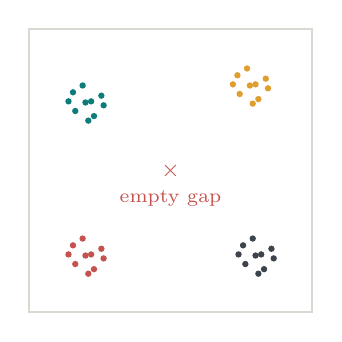
\begin{tikzpicture}[scale=0.72]
  \draw[hair, line width=0.8pt] (0,0) rectangle (5,5);
  % four tight, separated clusters with large empty gaps between them
  \foreach \cx/\cy/\col in {1/3.7/teal, 3.9/4/amber, 1/1/redd, 4/1/inksoft}{
    \foreach \dx/\dy in {0/0, 0.28/0.12, -0.22/0.18, 0.15/-0.24, -0.18/-0.15,
                         0.32/-0.05, -0.05/0.30, 0.10/0.02, -0.30/0.02, 0.05/-0.32}{
      \fill[\col] ($(\cx,\cy)+(\dx,\dy)$) circle (1.6pt);
    }
  }
  \node[redd, font=\footnotesize\bfseries] at (2.5,2.5) {$\times$};
  \node[redd, font=\scriptsize] at (2.5,2.0) {empty gap};
\end{tikzpicture}}
\newcommand{\latentB}{%
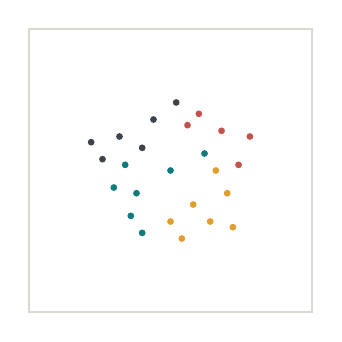
\begin{tikzpicture}[scale=0.72]
  \draw[hair, line width=0.8pt] (0,0) rectangle (5,5);
  % one broad, gap-free cloud; colours blend continuously
  \foreach \dx/\dy/\col in {%
    0/0/teal, 0.6/0.3/teal, -0.5/0.4/inksoft, 0.4/-0.6/amber, -0.6/-0.4/teal,
    0.9/0.7/redd, -0.9/0.6/inksoft, 0.7/-0.9/amber, -0.7/-0.8/teal, 1.2/0.1/redd,
    -1.2/0.2/inksoft, 0.1/1.2/inksoft, 0.2/-1.2/amber, 1.0/-0.4/amber, -1.0/-0.3/teal,
    0.3/0.8/redd, -0.3/0.9/inksoft, 0.8/0.0/amber, -0.8/0.1/teal, 0.0/-0.9/amber,
    1.4/0.6/redd, -1.4/0.5/inksoft, 0.5/1.0/redd, -0.5/-1.1/teal, 1.1/-1.0/amber}{
    \fill[\col] ($(2.5,2.5)+(\dx,\dy)$) circle (1.7pt);
  }
\end{tikzpicture}}

\begin{document}

\begin{center}
{\Large \textbf{Quiz 11 --- Learning Without (Many) Labels}}\\[2pt]
{\normalsize Predict what a latent samples to, use every spectrum, spot the reconstruction-error trap, and pick the augmentation that would corrupt contrastive pretraining}
\end{center}

\vspace{-2pt}
\begin{center}
\fbox{\parbox{0.92\textwidth}{\small
\textbf{Instructions:}\; Answer all four questions --- every part is answerable from the
pictures and rules on the slides. Intuition first; the only arithmetic is a mean of three
squared numbers. No calculators needed.%
\ifsolution\else\\[4pt]\textbf{Name:}\ \blk{6cm}\hfill\textbf{Date:}\ \blk{3.5cm}\fi
}}
\end{center}

\vspace{-2pt}\hrule\vspace{5pt}

% =========================== Q1 ===========================
\textbf{1. Sample each latent --- what decodes?}\; {\small Below are two latent-space maps of the
\emph{same} spectra --- the pair you saw on the slides. You want to \textbf{generate synthetic
resistant spectra} to augment training, so you sample a \emph{random} latent point and decode it.}

\vspace{4pt}
\begin{center}
\begin{tabular}{cc}
\latentA & \latentB \\[2pt]
\textbf{Picture A} & \textbf{Picture B}
\end{tabular}
\end{center}

\vspace{2pt}
\textbf{(a)} Sample \& decode a random point from \textbf{Picture A} (islands with gaps) --- what
comes out, and why?\hfill $\rightarrow$\; \rb{garbage (lands in an empty gap)}{5.6cm}

\vspace{3pt}
\textbf{(b)} Sample \& decode from \textbf{Picture B} (one smooth cloud) --- what comes out?
\hfill $\rightarrow$\; \rb{a plausible spectrum}{5.0cm}

\vspace{3pt}
\textbf{(c)} Which picture is the \textbf{VAE}, and which latent do you use to generate?
\hfill $\rightarrow$\; \rb{Picture B (the VAE)}{4.4cm}

\work{0.4cm}

\keybox{(a) \textbf{Garbage / a non-physical spectrum.} Picture A is a plain autoencoder: its
latent is scattered islands with big empty \textbf{gaps}, so a random sample lands where the
decoder was never trained. (b) \textbf{A plausible spectrum} --- Picture B is one smooth,
gap-free cloud, so \emph{every} point decodes to something realistic. (c) \textbf{Picture B is
the VAE}, and it is the latent you sample to generate (or interpolate): only a gap-free latent
is safe to sample. (B is also the map you would trust to flag a \emph{novel} contaminant --- a
genuinely new spectrum lands outside the tidy cloud, easy to flag.)}

\vspace{2pt}\hrule\vspace{5pt}

% =========================== Q2 ===========================
\textbf{2. Use every spectrum --- decide.}\; {\small You have \textbf{300 labelled} spectra
(susceptible/resistant known) and \textbf{40{,}000 unlabelled} QC runs, and you want a resistance
classifier. Use the four-paradigm chart from the slides.}

\vspace{4pt}
\textbf{(a)} Which paradigm uses \emph{all} of your data?\hfill $\rightarrow$\;\rb{semi-supervised}{4.6cm}

\vspace{3pt}
\textbf{(b)} Name the specific technique.\hfill $\rightarrow$\;\rb{pseudo-labelling}{4.6cm}

\vspace{3pt}
\textbf{(c)} In one sentence, the \emph{failure mode} to watch?

\work{1.0cm}
\ifsolution\else\blk{\linewidth}\fi

\keybox{(a) \textbf{Semi-supervised} --- a few labels plus many unlabelled examples, so use both
(the middle path). (b) \textbf{Pseudo-labelling}: train a first model on the 300 labelled,
predict on the 40{,}000 unlabelled, keep only the \emph{confident} predictions as pseudo-labels,
and retrain on the combined set (optionally repeat). (c) \textbf{Confident-but-wrong pseudo-labels
reinforce the model's own mistakes} --- a weak early model can poison the pool, so the confidence
filter matters. (Pure supervised would throw away 40{,}000 runs; pure unsupervised would ignore
the 300 labels you paid for.)}

\vspace{2pt}\hrule\vspace{5pt}

% =========================== Q3 ===========================
\textbf{3. Reconstruction error --- the aggregation trap.}\; {\small An autoencoder trained on
\emph{good} runs reconstructs a new spectrum of \textbf{20 $m/z$ bins}. A contaminant spikes
exactly \textbf{one} bin: that bin's squared error is \textbf{0.40}; the other \textbf{19} bins
reconstruct perfectly (error 0). Reconstruction error is the \emph{mean} squared error}
\[
  \text{MSE} \;=\; \tfrac{1}{n}\sum_{i}\,(x_i-\hat{x}_i)^2 ,
  \qquad\text{{\small flag an \textbf{anomaly} if the error } } > 0.05 .
\]

\vspace{2pt}
\textbf{(a)} MEAN over all 20 bins: $\text{MSE} = 0.40 / 20 = $ \rb{$0.02$}{2.0cm}

\work{0.4cm}

\textbf{(b)} Using the \emph{mean} and threshold $0.05$, does it flag the run?
\hfill $\rightarrow$\; \rb{no --- $0.02 < 0.05$, it PASSES}{5.4cm}

\work{0.4cm}

\textbf{(c)} The mean just \emph{missed} a real contaminant. Which \emph{single} number would have
caught it, and why does averaging hide a one-bin spike?

\work{1.1cm}
\ifsolution\else\blk{\linewidth}\\[6pt]\blk{\linewidth}\fi

\keybox{(a) $\text{MSE}=0.40/20=\mathbf{0.02}$. (b) \textbf{No} --- $0.02 < 0.05$, so the mean-MSE
\textbf{passes} the run and the contaminant slips through. (c) The \textbf{MAX per-bin error}
($0.40 > 0.05$), or the error inside the peak window, would flag it. The mean divides one big
error across 20 bins, so a \emph{localized} spike is diluted below threshold --- over thousands of
real $m/z$ bins a single contaminant peak can vanish into the average. Lesson: match the anomaly
\emph{score} to the anomaly's shape, and set the threshold as the same sensitivity/specificity
dial as Lecture~10.}

\vspace{2pt}\hrule\vspace{5pt}

% =========================== Q4 ===========================
\textbf{4. Which augmentation would corrupt it?}\; {\small Contrastive pretraining forces two
\emph{augmented views} of the \emph{same} spectrum to land at the \textbf{same} point in embedding
space. Three of the augmentations below are fine; \textbf{one} would corrupt the training.}

\vspace{3pt}
Mark each \textbf{SAFE} or \textbf{CORRUPT}:

\vspace{2pt}
(a) add random intensity noise $\rightarrow$ \rb{SAFE}{2.6cm} \qquad
(b) shift the $m/z$ axis by $0.2$ Da $\rightarrow$ \rb{SAFE}{2.6cm}

\vspace{2pt}
(c) replace it with a \emph{different} patient's spectrum $\rightarrow$ \rb{\textbf{CORRUPT}}{2.6cm} \qquad
(d) scale all intensities by $\times 1.05$ $\rightarrow$ \rb{SAFE}{2.6cm}

\vspace{3pt}
Which one is corrupt, and in one sentence, what would forcing agreement then teach the model?

\work{1.0cm}
\ifsolution\else\blk{\linewidth}\\[6pt]\blk{\linewidth}\fi

\keybox{\textbf{(c) is corrupt}; (a), (b) and (d) are safe. A valid augmentation adds only the
\emph{nuisance} variation the SAME sample would show run-to-run --- detector noise, a small $m/z$
calibration drift, a global intensity rescale --- so forcing those views to agree makes the model
\textbf{ignore the nuisance and keep the real content} (augmentation-invariance). But (c) is a
\emph{genuinely different sample}: forcing its embedding to match would teach the model to
\textbf{ignore real biological differences} --- it would treat two different patients as identical.
Rule: augmentations must preserve the underlying biology.}

\vspace{4pt}\hrule\vspace{3pt}
{\small\itshape \ifsolution Answer key.\else Keep this sheet --- Lab 4 trains a real VAE on
spectra, scores anomalies by reconstruction error, and plots the latent map.\fi}

\end{document}
